\documentclass[ngerman]{report}

\usepackage{../style}
\usepackage{fancyhdr}
\usepackage{tikz-cd}
\title{Einführung in die Funktionentheorie und Gewöhnliche Differentialgleichungen SS24}
\author{Raphael Frey, Benni Kleisz}
\institute{Universität Tübingen}
\department{Mathematik}
\date{\today}


\fancypagestyle{myfancystyle}{
  \fancyhf{}
  \fancyhead[L]{
    \begin{minipage}{1em}
        \rule[-1em]{1pt}{3em}
    \end{minipage}
    \begin{minipage}{\textwidth-2em}
        \emph{Aufgaben Funktionentheorie und Gewöhnliche Differentialgleichungen}\\
        \textbf{Sommersemester 2024}\\
        Raphael Frey, Benni Kleisz
    \end{minipage}
    }
  \renewcommand{\headrulewidth}{0pt}
  \renewcommand{\footrulewidth}{0pt}
}
\setlength{\headsep}{4em}
\pagestyle{myfancystyle}

\begin{document}
    \maketitle
    \begin{question}
        Identifiziere $\C = \R^2$ in üblicher Weise $(x + i y \equiv (x, y))$. Zeigen Sie: Ein $\R$-lineares $\varphi : \R^2 \to \R^2$ ist genau dann $\C$-linear, wenn $\varphi$ bzgl. der Standardbasis von $\R^2$ repräsentiert wird durch eine Matrix der Form 
        \begin{align*}
            \begin{pmatrix}
                a & -b\\
                b & a
            \end{pmatrix}, \quad a,b\in \R
        \end{align*}
        Durch welche komplexe 'Matrix' wird $\varphi$ dann repräsentiert?
    \end{question}
    \begin{answer}
        Die Äquivalenz der Bedingungen kann man in dem Kommutativen Diagramm \cref{fig:kommutatives_diagramm}
        \begin{figure}
            \centering
            \begin{tikzcd}
                \C^\ast \arrow{d}{\rho} &\C\arrow{l}{\alpha}\\
                M & \R^2\arrow{l}{\Phi}\arrow{u}{\Psi}
                \end{tikzcd}
            \caption{Isomorphismus $\C^\ast$ und $M$}
            \label{fig:kommutatives_diagramm}        
        \end{figure}
        Erkennen. Dabei ist $\alpha$ die kanonische Identifikation mit dem Produkt, $\Psi$ die kanonische Identifikation $\C\cong \R^2$ und $\Phi$ der lineare Isomorphismus ($M = \im\Phi$)
        \begin{align*}
            \Phi: \R^2 &\to M: (x,y)^t\mapsto \begin{pmatrix}
                x & -y\\
                y & x
            \end{pmatrix}.
        \end{align*}
        Es folgt mit $\rho$ als der Isomorphismus so, dass das Diagramm kommutiert, dass noch zu zeigen ist
        \begin{align*}
            \rho(\varphi) &= M_\varphi.
        \end{align*}
        Dies folgt durch $\alpha^{-1} \varphi = a+ib\in\C$,
        \begin{align*}
            \rho(\varphi) = \Phi \Psi^{-1}\alpha^{-1}\varphi = \Phi \Psi^{-1}(a+ib) = \Phi
            \begin{pmatrix}
                a\\
                b
            \end{pmatrix}
             = \begin{pmatrix}
                a & -b\\
                b & a
            \end{pmatrix}
        \end{align*} 
        und
        \begin{align*}
            M_\varphi = \left(\Psi \varphi\Psi^{-1}\begin{pmatrix}
                1\\
                0
            \end{pmatrix},\Psi \varphi\Psi^{-1}\begin{pmatrix}
                0\\
                1
            \end{pmatrix}\right) = \Biggl(\Psi \underbrace{\alpha\alpha^{-1}\varphi\Psi^{-1}\begin{pmatrix}
                1\\
                0
            \end{pmatrix}}_{(a+ib)\cdot 1},\Psi \underbrace{\alpha\alpha^{-1}\varphi\Psi^{-1}\begin{pmatrix}
                0\\
                1
            \end{pmatrix}}_{(a+ib)\cdot i}\Biggr) = \begin{pmatrix}
                a & -b\\
                b & a
            \end{pmatrix}. 
        \end{align*}
        Die repräsentierende komplexe Matrix ist also $\begin{pmatrix}a+ib\end{pmatrix}$.
    \end{answer}
    \begin{question}\hspace{\textwidth}
        \begin{enumerate}
            \item Zeigen Sie, dass die Funktion $f : \C \to \C$
            \begin{align*}
                f(z) = \begin{cases}
                    z^2 & z\in \R\\
                    z^3 & z\in \C\setminus\R
                \end{cases}
            \end{align*}
            komplex differenzierbar in $z_0=0$ ist mit $f'(0)=0$, aber nicht holomorph (d.h.es gibt keine Umgebung von $0$,auf der $f$ komplex diffbar ist).
            \item Skizzieren Sie den Verlauf von $f : \R \to \R$,
            \begin{align*}
                f(x) &= \begin{cases}
                    0 &, x= 0\\
                    \exp\left(-\frac{1}{x^2}\right), & x\neq 0
                \end{cases}
            \end{align*}
            (z.B. mit Hilfe von GeoGebra) und zeigen Sie: $f$ ist beliebig oft differenzierbar und $f^{(k)}(0) = 0$ für alle $k\in\N_0$ (Sie dürfen verwenden, dass $e^x$ schneller wächst als jede Potenz $x^n$,$n\in\N$).Folgern Sie, dass die Taylorreihe von $f$ in $0$ die Nullreihe ist und dass sie für $x \neq 0$ nicht gegen $f$ konvergiert.

        \end{enumerate}
    \end{question}
    \begin{answer}
        \begin{enumerate}
            \item Die Funktion ist komplex differenzierbar da (In einer Umgebung der $0$)
            \begin{align*}
                0\leq \abs{\frac{f(h)-f(0)}{h}} = \abs{\frac{f(h)}{h}}\leq \abs{\frac{h^2}{h}} = \abs{h} \to 0\implies f'(0) = 0
            \end{align*}
            Die Funktion kann nicht holomorph sein, da in $\R\setminus\{0\}$ die Funktion nicht stetig ist (Und $U_\varepsilon(0)\cap\R\neq\emptyset$). Sei $x \in \R\setminus\{0\}$
            \begin{align*}
                f\left(x+\frac{i}{n}\right) \to x^3\neq f(x) = x^2
            \end{align*}
            \item Die Funktion $f$ kann geschrieben werden als
            \begin{align*}
                p \cdot (\exp\circ q)
            \end{align*} 
            wobei $p,q \in \R[X^{-1}]$. Da $\R[X^{-1}]$ eine unter der (formalen) Ableitung abgeschlosse Unteralgebra der Laurentpolynome bildet, folgt für die $k+1$-te Ableitung 
            \begin{align*}
                \pder{x}f^{(k)}(x) = p'_k\cdot (\exp\circ q)+p_k\cdot q'\cdot (\exp\circ q) = (p_k'+p_k\cdot q')\cdot (\exp\circ q) = p_{k+1}\cdot(\exp \circ q)
            \end{align*} 
            Nach Induktion folgt (mit Induktionsanfang $f^{(0)}$) nun die Form 
            \begin{align*}
                p_k \cdot (\exp\circ q)
            \end{align*} 
            für $f^{(k)}$. Diese Ableitung kann stetig fortgesetzt werden mit 
            \begin{align*}
                \lim_{x\to 0} p_k(x) \cdot (\exp\circ q)(x) = 0 = f^{(k)}(0).
            \end{align*}
            Es folgt unmittelbar die Potenzreihe
            \begin{align*}
                \sum_{k=0}^\infty \frac{0}{k!}x^k = 0
            \end{align*}
            Und daraus folgt, da $\forall x\neq 0:f\neq 0$, dass die Taylorreihe außerhalb der $0$ nicht konvergiert
        \end{enumerate}
    \end{answer}
    \begin{question}
        Betrachten Sie für festes $c \in\R$ das Anfangswertproblem auf $\R^2$ 
        \begin{align*}
            y' &= y^2+1\\
            y(0) &= c                        
        \end{align*}
\begin{enumerate}
    \item Skizzieren Sie das Richtungsfeld. Können Sie evtl. eine Lösung raten? Dann testen Sie diese. 
    \item Lösen Sie das AWP nach "Trennung der Variablen" und geben Sie das (maximale) Existenzintervall an.
\end{enumerate} 
\end{question}
\begin{answer}\hspace{\textwidth}
\begin{enumerate}
    \item Das Richtungsfeld ist in \cref{fig:richtungsfeld.png} zu sehen. Eine wahrscheinliche lösung ist $y(x) = \tan x$. Es folgt
    \begin{align*}
        (\tan x)' = \frac{1}{\cos^2 x} = \frac{\sin^2 x}{\cos^2 x} + \frac{\cos^2 x}{\cos^2 x}= \tan^2 x+1
    \end{align*}
    \begin{figure}
        \centering
        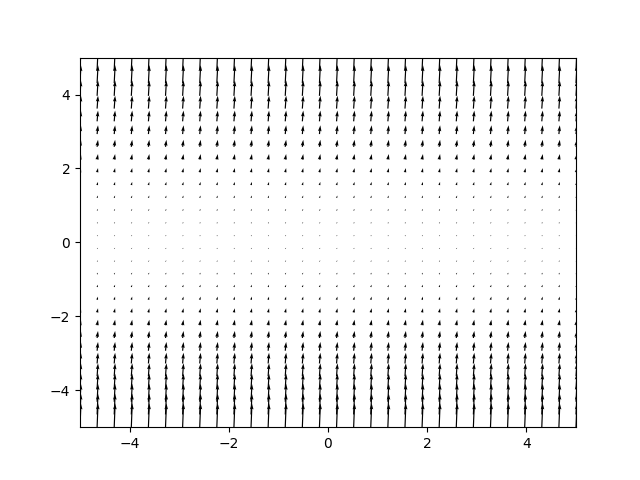
\includegraphics[width=\textwidth]{../figures/01-richtungsfeld.png}
        \caption{Richtungsfeld}
        \label{fig:richtungsfeld.png}
    \end{figure}
    \item Durch ''Trennung der Variablen'' folgt
    \begin{align*}
        \der[y]{x} = y^2+1 \implies \int \dif x = \int\frac{1}{y^2+1}\dif y \implies x+k = \arctan y \implies y = \tan (x+\arctan c)
    \end{align*}
\end{enumerate}
\end{answer}
    
\end{document}